
\documentclass[tikz]{standalone}
\usepackage{graphicx}
\usepackage{lmodern}
\usepackage{amsmath, amssymb, amsfonts}
\usetikzlibrary{calc}
\newcommand{\R}{\mathcal{R}}

\begin{document}

%t example
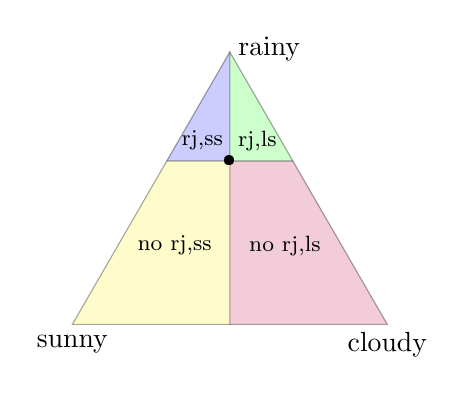
\begin{tikzpicture}
\draw[opacity = 0.2] (2,0) -- (-2,0) -- (0,3.46) -- cycle;
%label outcomes
\node at (-2, -0.25) {sunny};
\node at (1/2, 3.5) {rainy};
\node at (2, -0.25) {cloudy};
%level sets

\draw[fill = blue, fill opacity = 0.1, opacity = 0.2] (0, 3.46) -- (-0.8, 2.076) -- (0, 2.076) -- cycle; 
\node at (-0.35, 1.73*1.35) {\footnotesize rj,ss};
\draw[fill = green, fill opacity = 0.1, opacity = 0.2] (0, 3.46) -- (0.8, 2.076) -- (0, 2.076) -- cycle; \node at (0.35, 1.73*1.35) {\footnotesize rj,ls};

\draw[fill = yellow, fill opacity = 0.1, opacity = 0.2] (-2,0) -- (-0.8, 2.076) -- (0, 2.076) -- (0,0) -- cycle; \node at (-0.7, 1) {\footnotesize no rj,ss};
\draw[fill = purple, fill opacity = 0.1, opacity = 0.2] (2,0) -- (0.8, 2.076) -- (0, 2.076) -- (0,0) -- cycle; \node at (0.7, 1.) {\footnotesize no rj,ls};

\node at (0,2.076) {\textbullet};

\end{tikzpicture}



\end{document}
%%% Local Variables:
%%% mode: latex
%%% TeX-master: t
%%% End:
